\newpage
\chapter{1D Fourier Flow}

The one-dimensional heat equation is one of the simplest partial differential equations and can be solved analytically. It is given by,

\begin{equation}
	\frac{\partial u}{\partial t} = \frac{\partial^2 u}{\partial x^2}
\end{equation}

\no where $u$ is the temperature field. The steady-state solution will always be a linear function between the two boundary temperatures. Simulations have been performed using SPARTA to obtain the solution to this heat equation for higher Knudsen numbers.

\section{Setup}

\begin{figure}[H]
  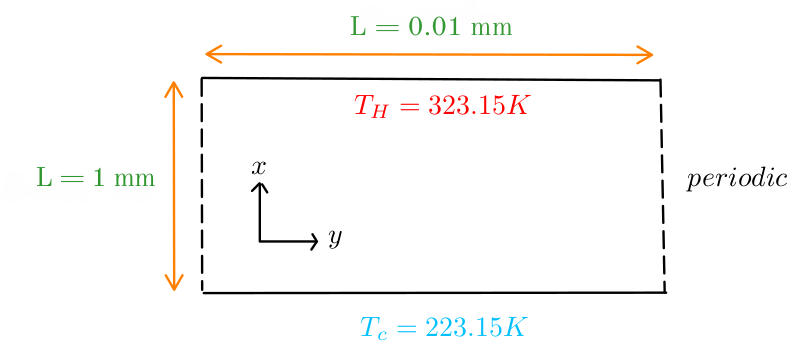
\includegraphics[scale=0.5]{Pictures/Chapter_5_1D_Fourier_Flow/Setup.png}
  \centering
  \caption{Setup of the simulation}
  \label{img:domain}
\end{figure}

For all the simulations, the gas is chosen to be Argon, with a molecular mass of $m = 6.63 \times 10^{-26} kg$ and a diameter of $d = 3.658 \times 10^{-10} m$. The simulation domain is chosen as given in Figure \ref{img:domain}. Since SPARTA doesn't have support for 1D simulations, the choice of the domain is made such that the $x$-direction is much larger than the $y$-direction, to approximate the domain as 1 dimensional. \\

\no At the mean temperature between $T_C$ and $T_H$, the most probable speed of the molecules is obtained using the expression given below,

\begin{equation} \label{eq:v_mps}
	v_{mps} = \sqrt{\frac{2 k_B T}{M}}
\end{equation}

\no where $k_B = 1.38 \times 10^{-23} J/K$ is the Boltzmann constant, $T$ is the temperature of the particle and $M$ is the molecular mass of the particle. Substituting for these values, we get the most probable speed for Argon under the conditions of the simulation is $v_{mps} \approx 337.208 m/s$. The mean free path for a monoatomic molecule is given by,

\begin{equation} \label{eq:mean_free_path}
	\lambda = \frac{1}{\sqrt{2}\pi n d^2}
\end{equation}

\no where $n$ is the number density of the particle in the domain and $d$ is the molecular diameter of the particle. Substituting the value of $d$ in the expression, we obtain, 

\begin{equation}
	\lambda \approx \frac{1.682 \times 10^{18}}{n}
\end{equation}

\no Using the expression for the Knudsen number given in Equation \ref{eq:kn}, we obtain,

\begin{equation}
	Kn = \frac{1.682 \times 10^{21}}{n}
\end{equation}

\no where $10^{-3} m$ is taken to be the characteristic length scale of the problem. To obatin a Knudsen number of 0.1, which is in the transitional regime, we must have $n =  1.682 \times 10^{22} kg/m^3$. Once the number density is known, we can find the number of particles in the domain $N$ using,

\begin{equation}
	N = n V
\end{equation}

\no where $V$ is the volume of the simulation domain. Since SPARTA takes the $z$-dimension to be 1 for 2D simulations, we obtain the volume as,

\begin{equation}
	V = \Delta x \Delta y \Delta z = \left( 10^{-3} \times 10^{-8} \times 1\right)  m^3 = 10^{-8} m^3 
\end{equation}

\no Consequently, the number of particles in the domain is calculated to be $N = 1.682 \times 10^{14}$. Similarly, the mean collision time can be calculated using,

\begin{equation} \label{eq:mean_coll_time}
	t_o =  \frac{\lambda}{v_{mps}}
\end{equation}

\no and this evaluates to $t_o \approx 2.966 \times 10^{-7} s$. We pick the grid cell size and time step size to keep them smaller than $\lambda$ and $t_o$ respectively, and will use $\tau = 10^{-8} s$ as the timestep and $(100 \times 1 \times 1) $ grid cells in the domain. \\

\no Now that the number of grid cells is fixed, we can calculate the number of simulated particles by picking the number of particles that each grid cell contains. Depending on the number of particles we pick, the simulations will be slightly different. I have selected two such numbers, 20 particles per grid cell and 100 particles per grid cell to see how the number of simulated particles affects the solution.

\section{Solution for 20 Particles per Grid Cell}

If we choose to have 20 particles per grid cell, and 100 grid cells in total, that implies that we have to use 2000 simulated particles in the simulation. Since the total number of particles is fixed, the simulation ratio can be found as $F_N = 8.41 \times 10^{10} $. The simulation is run for a million steps yielding a total physical time of 0.01 seconds. The parameter for convergence is chosen to be the global temperature. Plots of some representative time steps are highlighted below. All the plots and the video files showing the evolution of the system can be found in the repository containing the project \cite{Raghuveeran_Work_During_Summer_2024}.

\begin{figure}[H]
	\centering
    \includesvg[width=0.7\linewidth]{Pictures/Chapter_5_1D_Fourier_Flow/Temperature_0.010000_sec_20ppgc.svg}
    \caption{Solution obtained through SPARTA for 20 particles per grid cell}
	\label{gra:kn0.1_20ppgc_100g}
\end{figure}

\no We can clearly see that the temperature profile obtained through DSMC appears roughly linear, but the slope doesn't match the slope that is expected from the analytical solution. One can also see that the fluctuations in the solution are evident with there being random spikes in the solution. The reason for the slope not matching will be described in detail in the next few pages.

\section{Solution for 100 Particles per Grid Cell}

If we choose to have 100 particles per grid cell, and 100 grid cells in total, that implies that we have to use 10000 simulated particles in the simulation. Since the total number of particles is fixed, the simulation ratio can be found as $F_N = 1.682 \times 10^{10} $. The simulation is run for a million steps yielding a total physical time of 0.01 seconds. The parameter for convergence is chosen to be the global temperature. Plots of some representative time steps are highlighted below. All the plots and the video files showing the evolution of the system can be found in the repository containing the project \cite{Raghuveeran_Work_During_Summer_2024}.

\begin{figure}[H]
	\centering
    \includesvg[width=0.7\linewidth]{Pictures/Chapter_5_1D_Fourier_Flow/Temperature_0.010000_sec_100ppgc.svg}
    \caption{Solution obtained through SPARTA for 100 particles per grid cell}
	\label{gra:kn0.1_100ppgc_100g}
\end{figure}

\no We can clearly see that the temperature profile obtained through DSMC appears roughly linear, but once again, the slope doesn't match the slope that is expected from the analytical solution. One can also see that the fluctuations in this solution are much lesser than that in Figure \ref{gra:kn0.1_20ppgc_100g}. This is as expected. When we increase the number of simulated particles, the statistical fluctuations in the solution start to reduce.

\section{Deviation of the Solution from the Analytical Slope}

From Figures \ref{gra:kn0.1_20ppgc_100g} and \ref{gra:kn0.1_100ppgc_100g}, it is evident that at the temperature plates, the temperatures are different from what is actually applied. As a result, the slope of the solution also changes. The claim is that this is an effect due to the higher Knudsen number of the flow. To prove this conclusively, let's consider the following adjustments to the problem.

\subsection{Case 1 : Resolving the Grid}

Just to verify that the mismatching slopes is not due to the grid not being resolved sufficiently, let's resolve the grid to $(200 \times 1 \times 1)$ and see what happens to the solution. Considering the same 100 particles per grid cell to reduce fluctutations, the number of simulated particles will now become 20000. To keep the total number of physical particles the same, the simulation ratio $F_N$ will become $8.41 \times 10^9$. The plot of the temperature profile at the same instant but for 200 grid cells is given in Figure \ref{gra:kn0.1_100ppgc_200g}.

\begin{figure}[H]
	\centering
    \includesvg[width=0.7\linewidth]{Pictures/Chapter_5_1D_Fourier_Flow/Temperature_0.010000_sec_100ppgc_200g.svg}
    \caption{Solution obtained through SPARTA for 200 grid cells}
	\label{gra:kn0.1_100ppgc_200g}
\end{figure}

\no Notice how the solution in Figure \ref{gra:kn0.1_100ppgc_200g} resembles the solution in Figure \ref{gra:kn0.1_100ppgc_100g} almost identically. This allows us to conclude safely that the disparity in the slope is not due to the resolution of the grid.

\subsection{Case 2 : Changing the Knudsen Number}

Now to see that the disparity in the slopes is indeed an effect of rarefraction of the flow, we shall perform the simulation for a flow with a Knudsen number of 0.02. Since the knudsen number is decreased by a factor of 5, the number of particles must increase by a factor of 5. For 100 grid cells, and the same 100 particles per grid cell, the number of simulated particles is 10000. But to obtain the new Knudsen number of 0.02, the simulation ratio must be set to $F_N = 8.41 \times 10^{10}$. If we plot the solution at the same time step as the above solutions, we obtain Figure \ref{gra:kn0.1_100ppgc_kn_0.02}.

\begin{figure}[H]
	\centering
    \includesvg[width=0.7\linewidth]{Pictures/Chapter_5_1D_Fourier_Flow/Temperature_0.010000_sec_kn_0.02.svg}
    \caption{Solution obtained through SPARTA for $Kn = 0.02$}
	\label{gra:kn0.1_100ppgc_kn_0.02}
\end{figure}

\no Clearly, in Figure \ref{gra:kn0.1_100ppgc_kn_0.02}, the solution is a much closer match to the theoretical slope. This further strengthens the argument that the disparity in the slopes is a rarefraction effect that vanishes with decreasing the Knudsen number. In fact, this phenomenon is well known and the region around the boundary in which these deviations occur is called \textbf{knudsen layers}. Rader et al. (2005) also describe the effect of these Knudsen layers \cite{article}.